% !TeX root = root.tex
% !TeX spellcheck = en_US
\section{GAP-exercise}
\subsection*{a)}
For the group $G = \langle g_1,g_2,g_3,g_4 \rangle$ the GAP-function \textit{IsPrimitive} returns true and with the function \textit{ONanScottType} we get that $G$ is almost simple. Thus, $G$ is a primitive permutation group of almost simple type.

\subsection*{b)}
We use the following GAP code to get examples for the O'Nan-Scott types:

\lstinputlisting[language=gap]{ex4.g}

For affine type we get the group $\langle (1,2) \rangle$. 

For almost simple type we get $\langle (1,2,3,4,5) (3,4,5) \rangle$.

For diagonal type we get 

\hspace*{-1cm}
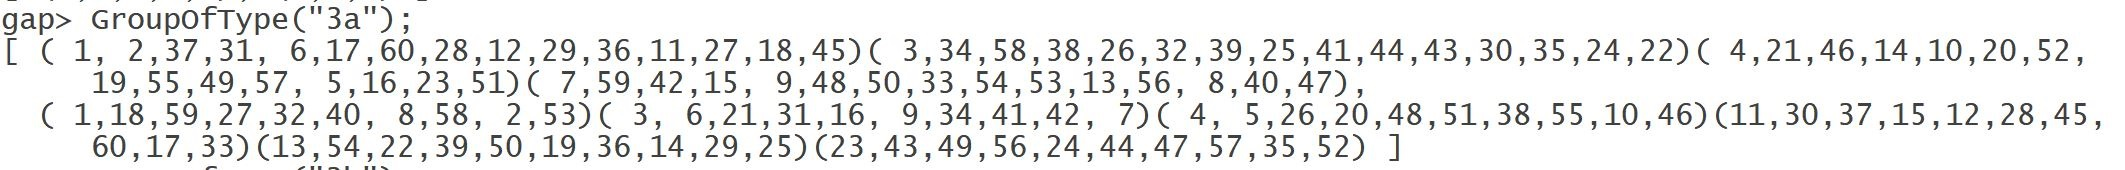
\includegraphics[width=17cm]{ex4_3}

For product action of wreath product we get

\hspace*{-1cm}
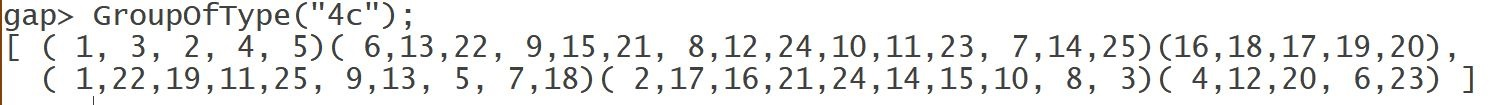
\includegraphics[width=17cm]{ex4_4}